\subsection{ROOTを用いたデータ解析}
MPPCで取得されるデータはEASIROCによってtree形式で保存される.
今回はこのデータをROOTを用いて解析を行う.
ここから解析に必要なROOTの知識を簡単に説明するが, すべてを説明することはできないため、わからない部分は各自調べるかTAに質問しよう.

特によく使われる目的としてはヒストグラム・グラフを描く, 任意の関数でフィットする, 大量のデータを処理するといったものがあります.
物理学実験では大量のデータを扱うため, 例えばエクセルのようなものではそれらのデータをプロットしたり複雑な解析を行うことは難しくなります.
そのため, プログラミングによる解析を行えるようになる必要となります.
言語としては主にC++で動作し, pythonで書くこともできます.

\subsubsection{ROOTの起動方法}
ROOTの起動方法はコマンドラインに以下のコマンドを入力するだけです.
\begin{lstlisting}
root
\end{lstlisting}
\begin{figure}[ht]
  \begin{center}
    \includegraphics[width=8cm]{../ROOT_logo.png}
    \caption{ROOTのロゴ}
    \label{fig:ROOT_logo}
  \end{center}
\end{figure}
起動の度に図\ref{fig:ROOT_logo}が表示されるため, オプションをつけます.
\begin{lstlisting}
root -l
\end{lstlisting}
\begin{table}[ht]
  \caption{ROOT起動時のオプションの例}
  \centering
  \begin{tabular}{lcr}
    \hline
    オプション & 意味                                           \\
    \hline \hline
    -l:        & 起動時にロゴを表示しない                       \\
    -b:        & ヒストグラムやグラフのグラフィックを描画しない \\
    -q:        & スクリプトファイルを実行後自動でROOTが終了する \\
    \hline
  \end{tabular}
\end{table}
ROOTを終了したいときには, .qと入力すればROOTを終了させることができる.

\subsubsection{ヒストグラムの描き方}
rootを起動する際に, 引数にrootファイルを指定することでrootの起動と同時にROOTファイルを開くことができる.例えば, 今回測定結果をexample.rootという名前で保存しているとした場合, root example.rootとコマンドラインから入力することで測定データに簡単にアクセスすることができる.\ref{fig:open_ROOT}
\begin{figure}[h]
  \begin{center}
    \includegraphics[width=8cm]{../SummerChallenge_open_root.png}
    \caption{rootファイルを開く}
    \label{fig:open_ROOT}
  \end{center}
\end{figure}

ファイルの中身をみると, こうなっているはず.

\begin{figure}[h]
  \begin{center}
    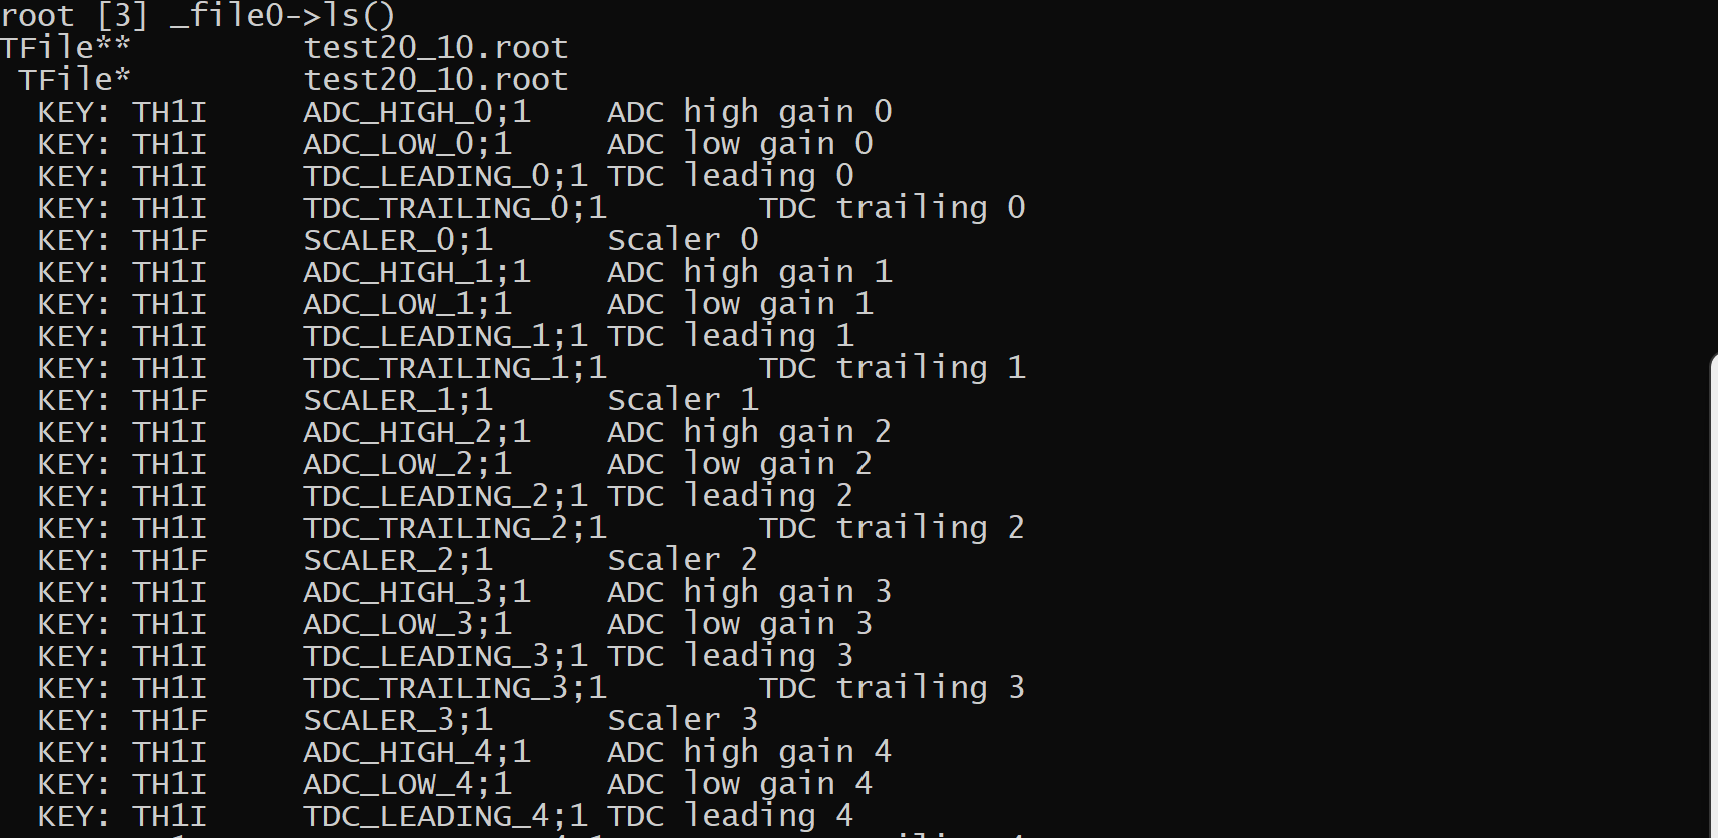
\includegraphics[width=8cm]{../SummerChallenge_ls_list.png}
    \caption{rootファイルの中身を確認する}
    \label{fig:ls_ROOT}
  \end{center}
\end{figure}

ADC$\_$HIGH$\_$12-$>$Draw() でヒストグラムを描くことができる.

\begin{figure}[h]
  \begin{center}
    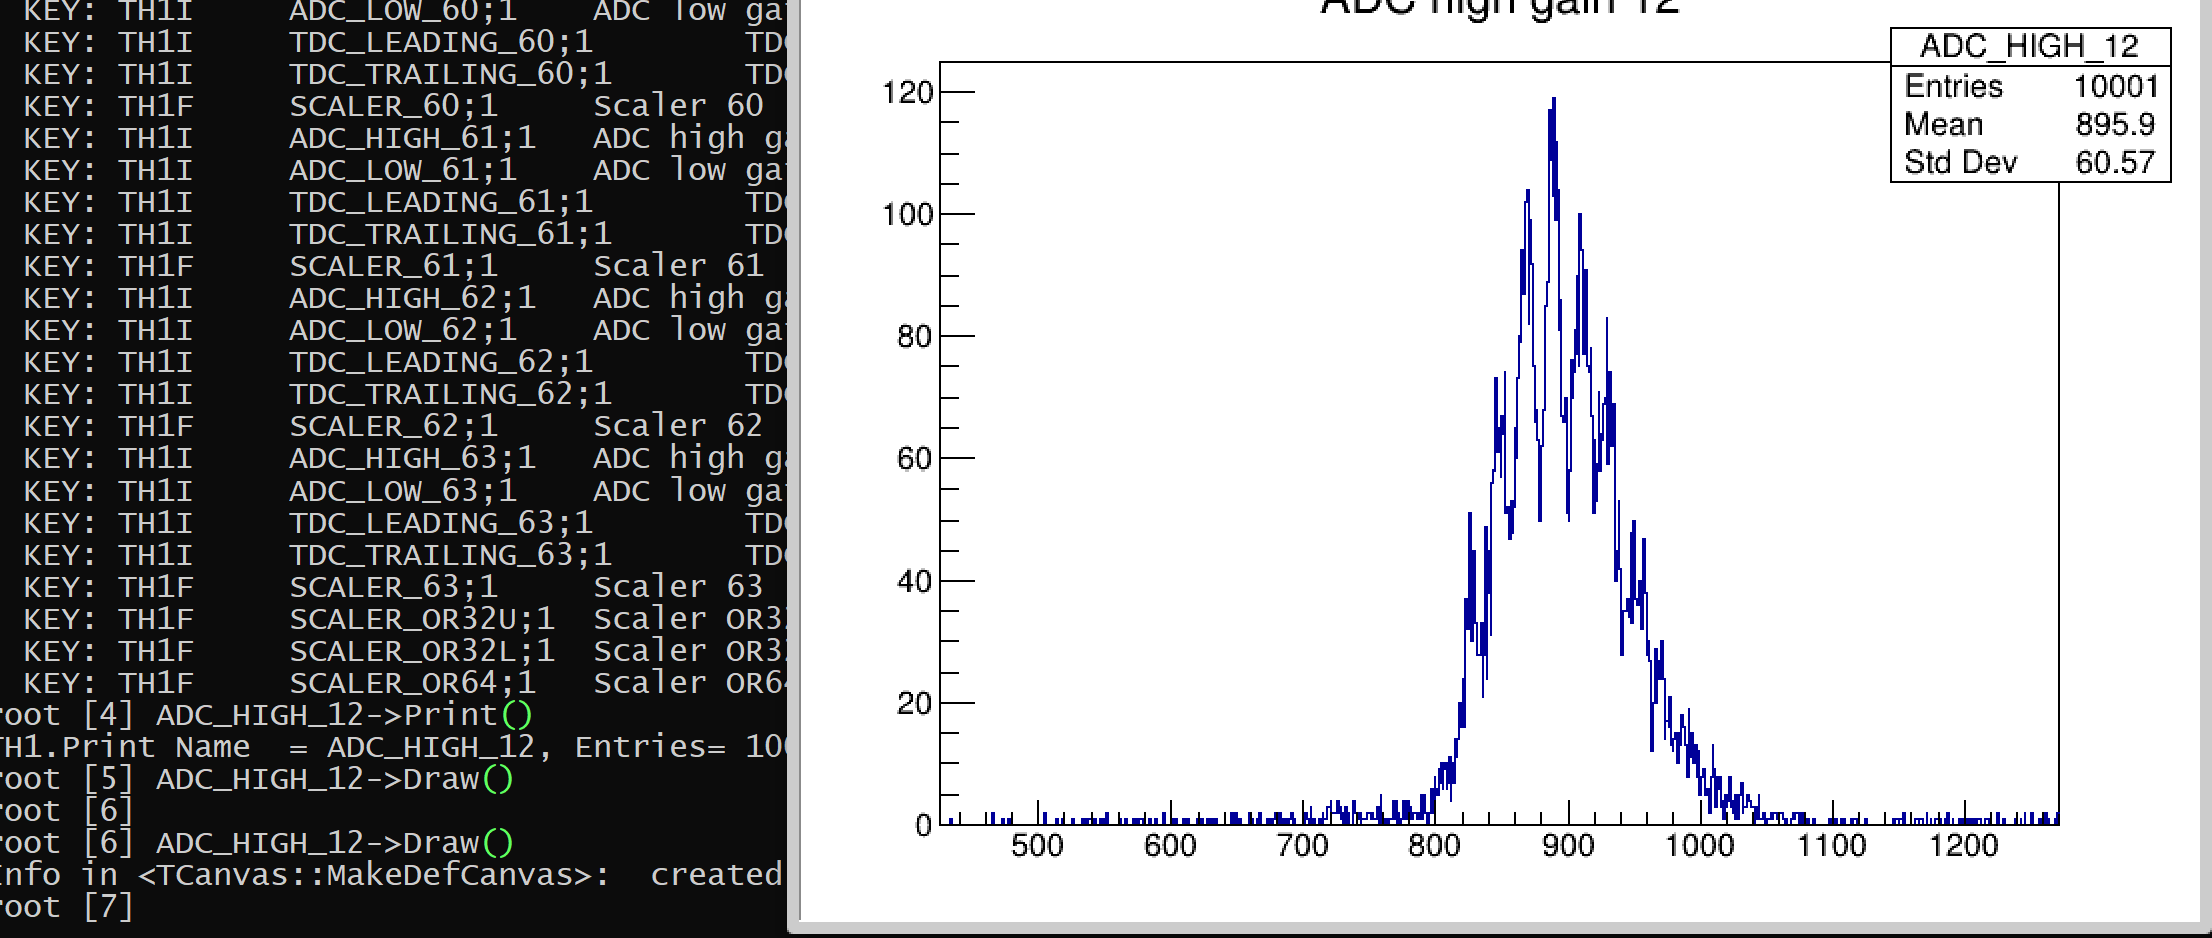
\includegraphics[width=8cm]{../SummerChallenge_draw_adc12.png}
    \caption{ヒストグラムを描く}
    \label{fig:ls_ROOT}
  \end{center}
\end{figure}

example.root内にさらにtreeという名前でtreeを作っている場合, tree-$>$"コマンド"という書き方をすることができる.それにより, 簡単に測定データを確認したりヒストグラムを描くことができる.コマンドとしては例えば, tree-$>$Print$\left(\right)$やtree-$>$Scan$\left(\right)$があり, Printはデータの数や種類, 変数の方を確認でき, Scanは1つ1つのデータを実際に確認することができる.
\begin{figure}[htbp]
  \begin{center}
    \begin{tabular}{c}

      \begin{minipage}{0.5\hsize}
        \begin{center}
          \includegraphics[clip, width=60mm]{../SummerChallenge_tree_print.png}
          \hspace{1.6cm} (a)tree-$>$Print$\left(\right)$の実行例
        \end{center}
      \end{minipage}

      \begin{minipage}{0.5\hsize}
        \begin{center}
          \includegraphics[clip, width=60mm]{../SummerChallenge_tree_scan.png}
          \hspace{1.6cm} (b)tree-$>$Scan$\left(\right)$の実行例
        \end{center}
      \end{minipage}
    \end{tabular}
  \end{center}
\end{figure}

今回treeの中身をPrintやScanで確認すると, いくつかのBranchがあると思う.\footnote{Branchとは言葉通り枝のようなもので, 1つのEntryに対して様々なデータを詰め込むことができる.}そのうち今回adcというBranchのヒストグラムを描きたい場合, tree-$>$Draw$\left("adc"\right)$と打つだけでヒストグラムを描くことができる.\footnote{今回, EASIROCでは32chのデータが配列としてadcのBranchに入っており, そのうちMPPCがつながっているのは30chのみなので, adc[30]のみをDrawすることで測定データのヒストグラムを描ける}
\begin{figure}[htbp]
  \begin{center}
    \begin{tabular}{c}

      \begin{minipage}{0.5\hsize}
        \begin{center}
          \includegraphics[clip, width=60mm]{../SummerChallenge_tree_draw_adc.png}
          \hspace{1.6cm} (a)tree-$>$Draw("adc")の実行例
        \end{center}
      \end{minipage}

      \begin{minipage}{0.5\hsize}
        \begin{center}
          \includegraphics[clip, width=60mm]{../SummerChallenge_tree_draw_adc30.png}
          \hspace{1.6cm} (b)tree-$>$Draw("adc[30]")の実行例
        \end{center}
      \end{minipage}
    \end{tabular}
    \label{fig:tree_draw}
  \end{center}
\end{figure}

ヒストグラムを書くときに, ただそのまま書くだけでなく様々な条件をかけることもできる.例えば, tree-$>$Draw("adc*2")とすれば, adcの値を2倍したヒストグラムを描くことができ, tree-$>$Draw("adc","adc$>$900")とすればadcが900より大きいイベントのみ描くことができます.この条件には, ほかのBranchを用いることもできtree-$>$Draw("adc","adc\_l $>$ 1000 \&adc\_l $<$ 3000")とすれば1000$<$adc\_l$<$3000のみのヒストグラムを描くことができる.ただし, ある程度複雑な条件になってくるとこの書き方をするのは難しくなってくるので, 後述するマクロを書いてヒストグラムを描くことをお勧めする.

最後にtreeをそのままdrawする以外のヒストグラムの描き方として, Fillという方法がある.簡単な例として, 自分でガウス分布に従う乱数を発生させてそれをヒストグラムに詰めるやり方を紹介する.
\begin{lstlisting}
    TH1D *h1 = new TH1D("h1","h1",50,-5,5);
    for(Int_t i = 0;i < 10000;i++){
     Double_t x = gRandom->Gaus();
     h1->Fill(x);
    }
    h1->Draw();
 \end{lstlisting}
3行目でgRandomというものを用いてGauss分布に従う乱数を発生させ, それを4行目でFillというコマンドでh1のヒストグラムに詰めている.それをfor文で回して10000回詰めている.このヒストグラムをDrawすることでGauss分布に従うヒストグラムを描くことができる.今回は例として乱数をFillしたが, 乱数の代わりに詰めたい値を詰めることで好きなヒストグラムを描くことができる.

\subsubsection{マクロの書き方}
簡単なマクロはコマンドラインに書いてヒストグラムを描くときと同じものを描くだけでよい.ただし, rootファイルを読み込む際には必要な手順があるので例としてそれを示す.
\begin{lstlisting}[basicstyle=\ttfamily\footnotesize, frame=single]
void macro(){
	TFile *file = new TFile("example.root");
	TH1D *h1 = (TH1D*)file->Get("adc");
	h1->Draw();
}
 \end{lstlisting}
というファイルを作り, ターミナル上でroot macro.cxxやrootを起動した後, .x macro.cxxとコマンドすることでこのマクロを実行できる.
データの解析には基本的にはROOT固有の知識はそれほど必要ではなく, c++の知識があれば充分であるため深くは説明しない.

もう一つ必要な知識として, 詳しい解析を行う際にはBranchのデータをヒストグラムとしてではなく値として取り出す必要がある.そのためこれも簡単にではあるが, 値としての取り出し方を説明する.

\begin{lstlisting}
void macro(){
    TFile *file = new TFile(inputfilename, "read");
    TTree *tree = (TTree*)file->Get("tree");

    Double_t adc[32]
    tree->SetBranchAddress("adc", &adc);

    const Int_t N = tin->GetEntries();
    for (Int_t ientry = 0; ientry < N; ientry++) {
     tree->GetEntry(ientry);
     cout<<ientry<<"   "<<adc[30]<<endl;
   }
}
 \end{lstlisting}

tree-$>$GetEntry(ientry)とすることで, ientry番目のイベントのadcを読み込んでおり, それをfor文で全イベント回すことで全データを読み込んでいる.今回のマクロではcoutで出力しているだけだが, その値をvectorや配列に詰めることで解析に用いることができる.

コマンドラインによる解析の仕方も一応説明しているが, 測定直後にデータを簡単に確認したいといった場合を除いてはマクロを用いればよい.また, データを確認する場合でもTBrowser\footnote{ROOTを起動した後, TBrowser tbと入力することでrootファイルの中身をヒストグラムとして簡単に見ることができる}が便利であるため, あまり使用頻度は高くないと思われる.

\subsubsection{ヒストグラムのフィット}
ROOTにはあらかじめガウス分布やポアソン分布などの様々な関数が用意されており, それらをヒストグラムのフィットを行う際に利用できる.例えばガウス分布でフィットする際には, htemp-$>$Fit("gaus")とすればよい.\footnote{htempの部分はその時のヒストグラムの名前に応じて適宜変える}コマンドラインで行った場合にはコマンドラインにfitの結果が出力される.
\begin{figure}[h]
  \begin{center}
    \includegraphics[width=8cm]{../SummerChallenge_fit_gaus.png}
    \caption{フィットの結果}
    \label{fig:fit_gaus}
  \end{center}
\end{figure}

ガウス分布の場合は, $(gaus)=(Constant)\times$exp$(-\frac{(x-(Mean))^2}{2(Sigma)^2})$で定義されている.それぞれの出力されるパラメータは関数によって異なるため, ほかの関数を用いる際は一度確認しておくとよい.
また, htemp-$>$Fit("gaus","","",min,max)とすることでフィットする範囲を制限することができる.

あらかじめ定義されている関数以外の関数を用いたい場合は自分で定義することができる.例えば直線でフィットしたい場合には, 
\begin{lstlisting}
TF1 *f1 = new TF1("f1","[0] + [1] * x",min,max);
 \end{lstlisting}
とすることでまず直線の関数を定義することができる.この関数の名前はf1になっているので, あとは先ほどガウス分布でフィットしたときと同様に, 
\begin{lstlisting}
htemp->Fit("f1","","",min,max);
 \end{lstlisting}
とすればよい.

フィットする際にある程度のパラメータを指定したい場合がある.その際にはf1-$>$SetParameter(0,5)とすれば0番目のパラメータの初期値を5に設定でき, f1-$>$SetParameters(5,10)とすればまとめて複数のパラメータの初期値を設定できる.

マクロで行う場合には基本的には同じだが, フィットした結果をマクロ内で用いたい場合は値として取り出す必要がある.
\begin{lstlisting}
Double_t p0 = f1->GetParameter(0);
 \end{lstlisting}
とすると, p0にフィットした後の0番目のパラメータの値を代入することができる.

\subsubsection{グラフの描き方}
基本的な使い方として, テキストファイルからグラフを描くやり方と配列やvector\footnote{vectorが何かわからない場合はc++の勉強が先に必要なため, c++ vector等で検索して使い方を勉強したほうがよいでしょう}を用いる方法がある.まずはテキストファイルでのグラフの書き方から説明する.

例としてdata.datというファイルに
\begin{lstlisting}
1.00 3936
0.50 3007
0.10 2249
-0.10 1836
-0.50 1097
-1.00 146
 \end{lstlisting}
と書かれている場合, 簡単にグラフを描くことができ
\begin{lstlisting}
TGraph *tg1 = new TGraph("data.dat");
tg1->Draw("AP");
 \end{lstlisting}
とするだけでグラフを描くことができる.ただし, この方法を用いるためには結果をまずdatファイルとして出力する必要があるため, あまり使うことはないだろう.

配列やvectorを用いる場合, まずは配列やvectorにデータを詰める必要があり, その部分は省略する.すでに値が詰まっていると仮定すると, 配列の場合は
\begin{lstlisting}
TGraph *tg1 = new TGraph(6,x,y);
tg1->Draw("AP");
 \end{lstlisting}
とすると, 6個のデータを含むグラフを描くことができる.しかし, 測定データによってグラフが何点あるかは異なる場合もあり, vectorを用いたほうが様々な場合に柔軟に用いることができ便利である.

vectorを用いた場合は
\begin{lstlisting}
TGraph *tg1 = new TGraph(x.size(),&(x.at(0)),&(y.at(0)));
tg1->Draw("AP");
 \end{lstlisting}
c++の知識がある人は, これを見てやってることは同じだとわかると思う.

また, グラフにエラーバーをつけたい場合も多いと思う.その場合はTGraphではなくTGraphErrorsを用いればよい.使い方はほとんど同じで, 
\begin{lstlisting}
TGraph *tg1 = new TGraph(6,x,x_error,y,y_error);
tg1->Draw("AP");
 \end{lstlisting}
の順番に引数がなっており, その通りにTGraphの時と同様に配列やvectorで与えればよい.

最後にグラフのフィットについてであるが, ヒストグラムの場合と全く同じであり例えば直線でフィットしたい場合には
\begin{lstlisting}
TF1 *f1 = new TF1("f1","[0] + [1] * x",min,max);
tg1->Fit("f1","","",min,max);
 \end{lstlisting}
とすればグラフを直線でフィットすることができる.

\subsubsection{結果の保存}
コマンドラインで結果のヒストグラムやグラフを保存する場合には, 左上のFileからSave Asを選ぶと名前を付けて保存することができる.マクロで実行している場合には, ヒストグラムやグラフを描く前に
\begin{lstlisting}
TCanvas *c1 = new TCanvas("c1","c1",1600,900);
 \end{lstlisting}
としてキャンバスを作っておき, ヒストグラムやグラフをDrawした後に
\begin{lstlisting}
c1->SaveAs("save name");
 \end{lstlisting}
とすることで保存することができる.保存する際にきれいにヒストグラムやグラフを整えた後, 保存したい人も多いと思う.rootはヒストグラムやグラフそれぞれに様々な修飾等が存在し, それをここで説明しているときりがないためまとめ\ref{sec:lastsection}にそれらが書かれているリンクを載せておく.

また, ヒストグラムを保存する際に画像としてでなくrootファイルにヒストグラムのまま保存することができる.実際に触ってみないとそのメリットは感じにくいかもしれないが, rootファイルの状態で保存することで, 保存した後にタイトルをつけたりbin幅を変えるといった加工が簡単に行える.そのため, 最終的にスライド等に用いる時以外はrootファイルで保存しておいたほうが便利かもしれない.具体的なやり方が書かれているサイトのリンクをここに載せておく.\footnote{\url{https://www-he.scphys.kyoto-u.ac.jp/member/n.kamo/wiki/doku.php?id=study:software:root:io}のWrite ・オブジェクトをファイルに書き込む, rootファイルを保存するを参考にしてもらえばよい.}なお, ヒストグラム等を保存する際は測定データのrootファイルとは別に保存用のrootファイルを作るようにしてください.測定データを上書きしてしまうリスクを避けるために, 測定データは読み込み専用で開く習慣をつけるためである.
